\documentclass[a4paper,10pt]{article}
\usepackage[utf8x]{inputenc}
\usepackage[serbian]{babel}

\usepackage[version=3]{mhchem} % Package for chemical equation typesetting
\usepackage[margin=2.5cm]{geometry}
\usepackage{siunitx} % Provides the \SI{}{} and \si{} command for typesetting SI units
\usepackage{graphicx} % Required for the inclusion of images
\usepackage{natbib} % Required to change bibliography style to APA
\usepackage{amsmath} % Required for some math elements 
\usepackage{subfig} % For multiple figures side-by-side
\usepackage{url} % For linking url's properly

\setlength\parindent{0pt} % Removes all indentation from paragraphs

%\usepackage{times} % Uncomment to use the Times New Roman font

%----------------------------------------------------------------------------------------
%	DOCUMENT INFORMATION
%----------------------------------------------------------------------------------------

\title{OPNA: Prvi projektni zadatak \\ Verižni razvoj} % Title

\author{Aleksa \textsc{Ilić}} % Author name

\date{\today} % Date for the report

\begin{document}

\maketitle % Insert the title, author and date

\begin{abstract}
    U radu će biti prikazana praktična realizacija konzolnog programa koji izvršava numeričku procenu verižnog razlomka sa arbitrarnom preciznošću i modularnošću ispisa
\end{abstract}

%----------------------------------------------------------------------------------------
%	SECTION: UVOD
%----------------------------------------------------------------------------------------

\section{Uvod}
\subsection{Opis problema}

Za zadati broj $\mathit{x}$ i opseg $\mathit{n}$ i $\mathit{m}$ formirati niz razlomaka $\frac{p}{q}$ gde imenilac q ispunjava 
$\mathit{n \leq q \leq m}$ tj. $\mathit{q = n, n+1, ..., m}$. Brojilac $\mathit{p}$ je zaokružen na najbliži ceo broj vrednosti $\mathit{x*q}$, gde je $\mathit{q = n, n+1, ..., m}$. Potom u prethodnom nizu razlomaka $\frac{p}{q}$ formirati:

\begin{itemize}
\item Racionalne aproksimacije I vrste;
\item Racionalne aproksimacije II vrste;
\item Razlomke $\frac{p}{q}$ sortirati po minimalnosti apsolutne greške $\left|\mathit{x-\frac{p}{q}}\right|$
\end{itemize}

Formirati i zapisati u verižnom zapisu za sve dobijene aproksimacije

\subsection{Definicije}
\label{definitions}
\begin{description}
\item[Verižni razlomak]
Izraz oblika $\mathit{x = a_0 + \frac{1}{a_1 + \frac{1}{a_2 + \frac{1}{a_3 + ...}}}}$ gde je $\mathit{a_0 \in Z}$ i $\mathit{a_i \in N (i \neq 0)}$. Prethodni izraz skraćeno zapisujemo $\mathit{x = [a_0;a_1,a_2, ...]}$.
\item[Racionalna aproksimacija I vrste]
Racionalni broj $\frac{p}{q}$ jeste najbolja racionalna aproksimacija prve vrste realnog broja $\mathit{\alpha}$ ako važi: $\left|\alpha - \frac{p}{q}\right| < \left|\alpha - \frac{r}{s}\right|$ za sve razlomke $\frac{r}{s} \neq \frac{p}{q}$ takve da $0 < s \leq q$
\item[Racionalna aproksimacija II vrste]
Racionalni broj $\frac{p}{q}$ jeste najbolja racionalna aproksimacija druge vrste realnog broja $\mathit{\alpha}$ ako važi: $\left|q\alpha - p\right| < \left|s\alpha - r\right|$ za sve razlomke $\frac{r}{s} \neq \frac{p}{q}$ takve da $0 < s \leq q$
\end{description} 
Date definicije preuzete iz rada \cite{ARTICLE:Verizni}.
 
%----------------------------------------------------------------------------------------
%	SECTION: OPIS REŠENJA
%----------------------------------------------------------------------------------------

\section{Opis rešenja}

Za realizaciju rešenja korišćen je programski jezik \textbf{C++17} zajedno sa najnovijom verzijom \textbf{Boost} biblioteka u trenutku pisanja ovog rada. Celokupan, dokumentovani izvorni kod dostupan je na autorovom github profilu \cite{WEBSITE:Github}.

\vspace{11pt}
Aktuelna verzija (v0.2.0) rešenja, sa podrazumevanim vrednostima veličine tipova, korišćena je za generisanje svih slika i računskih ispisa. Rešenje omogućava visoku preciznost pri numeričkom računu, a ona se može i dodatno povećati ukoliko korisnik to želi. Takođe, ispis rešenja je vrlo modularan te korisnik može, dodavanjem odgovarajućih prarametara, dobiti željeni ispis. Pregled svih parametara i podrazumevanih podešavanja dat je na Slici \ref{fig:version}. Parameter --inbetween omogućava računanje međuverižnih aproksimacija. Simbolom zvezda (*) označene su verižne aproksimacije.

\begin{figure}
\begin{center}
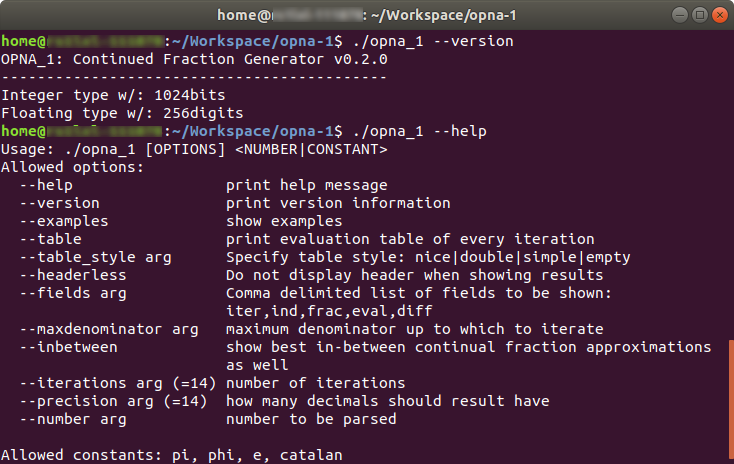
\includegraphics[width=0.9\textwidth]{version.png}
\caption{Podrazumevana podešavanja i pomoćni ekran}
\label{fig:version}
\end{center}
\end{figure}

\subsection{Primeri ispisa}

Na slikama \ref{fig:pi_example1} i \ref{fig:pi_example2} nalaze se primeri kojima se demonstrira verižno izračunavanje broja $\pi$. 
Ideja autora je da ovim primerom prikaže modularne sposobnosti ispisa, te neće biti analize samog numeričkog računa. 


Prva slika prikazuje tabelarni ispis do maksimalne veličine brojioca zadatim parametrom \textbf{--maxdenominator} dok drugi primer na to nadovezuje lični izbor i redosled kolona za prikaz (parametar \textbf{--fields}), njihov izgled (parametar \textbf{--table\_style}) i broj decimala koji se prikazuje (parametar \textbf{--precision}).

\begin{figure}
\begin{center}
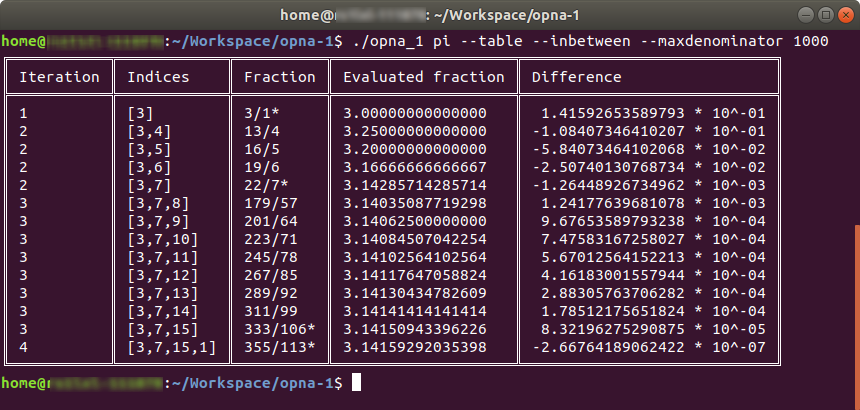
\includegraphics[width=0.9\textwidth]{pi_example1.png}
\caption{Tablearni ispis do maksimalnog brojioca}
\label{fig:pi_example1}
\end{center}
\end{figure}

\begin{figure}
\begin{center}
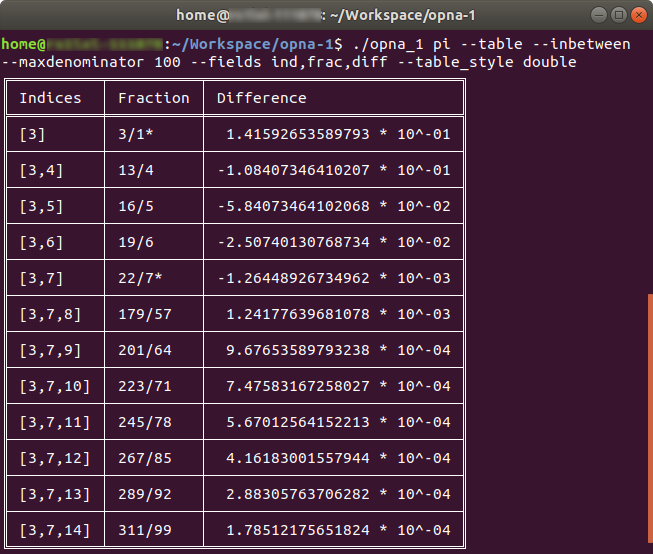
\includegraphics[width=0.9\textwidth]{pi_example2.png}
\caption{Različita korisnička podešavanja}
\label{fig:pi_example2}
\end{center}
\end{figure}

\newpage

%----------------------------------------------------------------------------------------
%	SECTION: RAČUN
%----------------------------------------------------------------------------------------

\section{Izračunavanje konstante \textit{G}}

Katalanova konstanta, \textit{G}, koja se javlja u kombinatorici definisana je kao:
\begin{equation}
\mathit{G} = \beta(2) = \sum_{n=0}^{\infty}\frac{(-1)^n}{(2n+1)^2} = 0.9159655941...
\end{equation}
gde je $\beta$ Dirihleova beta funkcija. Data definicija preuzeta je iz knjige \cite{BOOK:Constants}

\vspace{11pt}

Nepoznato je da li je \textit{G} iracionalan broj. Katalanova konstanta je dobila ime po \textit{Evgeniju Katalanu (30 May 1814 – 14 February 1894)}. Može se sračunati precizno i njena vrednost jednaka je $\pi^3/32$ 

\subsection{Podešavanja programa}
Za prikaz rešenja korišćene su podrazumevane veličine tipova, tabelarni prikaz uz \textit{simple} stil, sračunavanje do desete iteracije, uz prikaz 11 decimala. 

Autor se odlučio za tu preciznost jer nema smisla prikazivati više decimala za odlučeni broj iteracija što potvrđuje proračunata greška. 

\vspace{11pt}

Program je pokrenut dva puta. Prvi ispis prikazuje samo verižne aproksimacija, dok drugi ispis dodaje i međuverižne aproksimacije.

\vspace{11pt}

Rezultati će biti izneti u tekstualnom formatu kao proizvod izvršenja realizovanog programa sa pomenutim parametrima. Autor se odlučio za takav prikaz jer omogućava veću fleksibilnost u odnosu na sliku terminalnog prozora ukoliko čitalac želi da rezultate prekopira i koristi u svojim istraživanjima. Autor garantuje da svi brojevi odgovaraju ispisu programa i nisu na bilo koji način menjani, ali su neke međuverižne aproksimacije isečene zarad lepšeg ispisa.

\subsection{Rezultati}
\begin{verbatim}
 Indices                   Fraction       Evaluated fraction   Difference              
------------------------- -------------- -------------------- -------------------------
 [0]                       0/1*           0.00000000000         9.15965594177 * 10^-01 
 [0;1]                     1/1*           1.00000000000        -8.40344058228 * 10^-02 
 [0;1,10]                  10/11*         0.90909090909         6.87468508631 * 10^-03 
 [0;1,10,1]                11/12*         0.91666666667        -7.01072489448 * 10^-04 
 [0;1,10,1,8]              98/107*        0.91588785047         7.77437099293 * 10^-05 
 [0;1,10,1,8,1]            109/119*       0.91596638655        -7.92377402834 * 10^-07 
 [0;1,10,1,8,1,88]         9690/10579*    0.91596559221         1.96623499010 * 10^-09 
 [0;1,10,1,8,1,88,4]       38869/42435*   0.91596559444        -2.61334066128 * 10^-10 
 [0;1,10,1,8,1,88,4,1]     48559/53014*   0.91596559399         1.83179704684 * 10^-10 
 [0;1,10,1,8,1,88,4,1,1]   87428/95449*   0.91596559419        -1.44435481991 * 10^-11  
\end{verbatim}

\begin{verbatim}
 Indices                   Fraction       Evaluated fraction   Difference              
------------------------- -------------- -------------------- -------------------------
 [0]                       0/1*           0.00000000000         9.15965594177 * 10^-01 
 [0;1]                     1/1*           1.00000000000        -8.40344058228 * 10^-02 
 [0;1,5]                   5/6            0.83333333333         8.26322608439 * 10^-02 
 [0;1,6]                   6/7            0.85714285714         5.88227370344 * 10^-02 
 [0;1,7]                   7/8            0.87500000000         4.09655941772 * 10^-02 
 [0;1,8]                   8/9            0.88888888889         2.70767052883 * 10^-02 
 [0;1,9]                   9/10           0.90000000000         1.59655941772 * 10^-02 
 [0;1,10]                  10/11*         0.90909090909         6.87468508631 * 10^-03 
 [0;1,10,1]                11/12*         0.91666666667        -7.01072489448 * 10^-04 
 [0;1,10,1,5]              65/71          0.91549295775         4.72636430740 * 10^-04 
 [0;1,10,1,6]              76/83          0.91566265060         3.02943574809 * 10^-04 
 [0;1,10,1,7]              87/95          0.91578947368         1.76120493008 * 10^-04 
 [0;1,10,1,8]              98/107*        0.91588785047         7.77437099293 * 10^-05 
 [0;1,10,1,8,1]            109/119*       0.91596638655        -7.92377402834 * 10^-07 
 [0;1,10,1,8,1,44]         4894/5343      0.91596481378         7.80402186262 * 10^-07 
 [0;1,10,1,8,1,45]         5003/5462      0.91596484804         7.46136208396 * 10^-07 
 [0;1,10,1,8,1,46]         5112/5581      0.91596488085         7.13331492443 * 10^-07 
 [0;1,10,1,8,1,47]         5221/5700      0.91596491228         6.81896517261 * 10^-07 
 ...
 [0,1,10,1,8,1,86]         9472/10341     0.91596557393         2.02481986108 * 10^-08 
 [0,1,10,1,8,1,87]         9581/10460     0.91596558317         1.10032228391 * 10^-08 
 [0,1,10,1,8,1,88]         9690/10579*    0.91596559221         1.96623499010 * 10^-09 
 [0,1,10,1,8,1,88,3]       29179/31856    0.91596559518        -1.00108334557 * 10^-09 
 [0,1,10,1,8,1,88,4]       38869/42435*   0.91596559444        -2.61334066128 * 10^-10 
 [0,1,10,1,8,1,88,4,1]     48559/53014*   0.91596559399         1.83179704684 * 10^-10 
 [0,1,10,1,8,1,88,4,1,1]   87428/95449*   0.91596559419        -1.44435481991 * 10^-11 
\end{verbatim}

%----------------------------------------------------------------------------------------
%	SECTION: DISKUSIJA
%----------------------------------------------------------------------------------------

\section{Diskusija rezultata}

Program je kroz 10 iteracija došao do aproksimacije koja odgovara priloženoj definiciji konstante, na početku poglavlja 3. Međutim proračunato rešenje ($\frac{87428}{95449}$), nije toliko korisno za upotrebu usled njegove veličine. Autoru je znatno interesantnije verižno rešenje koje se dobija u 6. iteraciji ($\frac{109}{119}$) jer predstavlja optimalan odnos veličine i preciznosti. Evaluacija ove aproksimacije odstupa od konstante tek na 6. decimali.

%----------------------------------------------------------------------------------------
%	BIBLIOGRAPHY
%----------------------------------------------------------------------------------------

\bibliographystyle{apalike}

\bibliography{sample}

%----------------------------------------------------------------------------------------


\end{document}